\documentclass[journal,twocolumn]{IEEEtran}
\usepackage{amsmath,amsfonts,amssymb}
\usepackage{array}
\usepackage{textcomp}
\usepackage{url}
\usepackage{graphicx}
\usepackage{cite}
\usepackage{booktabs}
\usepackage{multirow}
\usepackage{xcolor}

% tighten spacing so 4-page budget holds
\setlength{\textfloatsep}{6pt plus 1pt minus 1pt}
\setlength{\floatsep}{6pt plus 1pt minus 1pt}
\setlength{\intextsep}{6pt plus 1pt minus 1pt}
\setlength{\abovedisplayskip}{3pt plus 1pt minus 1pt}
\setlength{\belowdisplayskip}{3pt plus 1pt minus 1pt}
\setlength{\abovecaptionskip}{3pt}
\setlength{\belowcaptionskip}{0pt}

\begin{document}

\title{Confidence-Routed Unified Accelerator for Edge Stereo--Monocular Fusion}

\author{Anonymous Authors%
\thanks{Manuscript submitted April 2026. Companion manuscript to a parallel transactions submission; this letter isolates the confidence-routing contribution.}}

\markboth{IEEE Computer Architecture Letters (submission)}%
{Anonymous: Confidence-Routed Unified Accelerator}

\maketitle

\begin{abstract}
Modern 3D-CNN stereo matchers dominate public benchmarks, yet, lacking global semantic context, they degrade on reflective, transparent, and occluded ill-posed regions and generalize poorly across domains in zero-shot. Vision-Transformer monocular models such as Depth-Anything-V2 (DA2)~\cite{yang2024da2} restore that context through rich high-level reasoning, but their $>$120\,GFLOPs/frame cost and lack of metric output preclude both real-time on-device deployment and absolute-distance applications. We bridge both gaps with an SGM-guided monocular--stereo fusion network: Semi-Global Matching contributes a metric anchor and a per-pixel PKRN confidence map, while a hardware-friendly EfficientViT-B1 residual head consumes a 7-channel input (RGB, aligned mono disparity, SGM disparity, PKRN, validity) to emit a final metric disparity. With hole-augmented training and end-to-end INT8 quantization-aware fine-tuning, the network reaches \textbf{1.14\,px EPE / 6.08\,\% D1} on KITTI --- 39\,\% below a heuristic confidence-blend baseline --- and beats the heuristic on all eight EPE/D1 metrics across KITTI, SceneFlow, ETH3D, and Middlebury, at both FP32 and INT8. We further realize the pipeline on a unified accelerator (32$\times$32 systolic array $+$ 16$\times$3$\times$3 depthwise ring $+$ weight streamer) whose PKRN Routing Unit reuses the same confidence signal to drive four otherwise-independent dataflow decisions: encoder token-merge, decoder INT4/INT8 precision mask, LS anchor selection, and residual-fusion gate. This delivers \textbf{40.47\,FPS/W/mm$^2$ EDAP} --- 3.4$\times$ over a vanilla DA2 $+$ LS pipeline and 1.48$\times$ over the same fusion pipeline without confidence routing --- at 12.95\,FPS end-to-end. INT4 weights remain within 0.3\,\% of FP32. On reflective and zero-shot cross-domain samples where pure-stereo accelerators degrade, the SGM--DA2 fusion preserves accuracy.
\end{abstract}

\begin{IEEEkeywords}
Stereo matching, monocular depth, confidence-driven architecture, systolic array, hardware accelerator, SGM, EfficientViT, mixed precision.
\end{IEEEkeywords}

\section{Introduction}
\label{sec:intro}
\IEEEPARstart{E}{dge} depth estimation for AR, robotics, and ADAS demands both metric accuracy and millisecond-scale throughput. Semi-Global Matching (SGM)~\cite{hirschmuller2008sgm} reaches millisecond latency on FPGAs and produces metric disparity, but fails on textureless, reflective, and occluded regions. Vision-Transformer monocular networks such as Depth-Anything-V2~\cite{yang2024da2} cover those regions robustly, but deliver only up-to-scale depth and cost tens of GFLOPs/frame, roughly $20\times$ more than an edge budget tolerates. Fusing the two is the natural design, and a stereo-matcher confidence score is the natural blending weight.

On the accuracy side, 3D-CNN stereo matchers (e.g., PSMNet~\cite{chang2018psmnet}, IGEV~\cite{xu2023igev}) dominate public benchmarks yet inherit the same ill-posed-region weakness, and their dense cost-volume processing pushes compute further beyond edge budgets. On the deployment side, recent low-power edge-stereo accelerators take an incremental path: they preserve the classical SGM/cost-aggregation skeleton and replace only its hand-crafted features with low-precision (fixed-point or binary) descriptors~\cite{zhao2020fpstereo}, achieving real-time FPS at the cost of a substantial accuracy gap to fully learned methods. We argue this incrementalism caps the achievable ceiling: rather than patching either side, we restructure the edge-stereo pipeline at the source so that a learned monocular network supplies high-level context where classical matching fails, and the classical confidence signal in turn steers the learned model's compute.

\textbf{Confidence is usually a terminal cue; we promote it to a control signal.} In prior stereo--mono fusion pipelines, the SGM confidence map enters the datapath only at the final output-combination stage~\cite{poggi2016pkrn,facil2019camconvs}; the rest of the pipeline either ignores it or recomputes an internal learned proxy~\cite{you2023vitcod,wang2021spatten}. We take a different position: the SGM per-pixel PKRN score, produced \emph{upstream of the accelerator for free} as a physical byproduct of the left--right check on the SGM cost volume, should be the single shared control input that drives every confidence-sensitive stage of the downstream pipeline. A small 4\,KB on-chip PKRN Routing Unit (PRU) applies four module-local transforms (threshold\,$+$\,pool, binarize, top-$k$, rescale) and broadcasts the results to four otherwise-independent dataflow decisions on one unified 32$\times$32 systolic fabric.

\textbf{Contribution.} We design, model, and evaluate a unified confidence-routed accelerator whose PRU couples four control decisions --- encoder token-merge plan, decoder INT4/INT8 precision mask, least-squares (LS) anchor selection, and residual-fusion gate --- onto one 32$\times$32 systolic array and one 16$\times$3$\times$3 depthwise ring. Compared against the no-routing variant of the same accelerator (row A$+$EV in Table~\ref{tab:cal1}), PKRN routing cuts latency 34\% and raises energy--delay--area product (EDAP) by 48\% while holding INT8 weight accuracy within 0.01\,px EPE of FP32 on KITTI.

\section{Background}
\label{sec:bg}
SGM aggregates a stereo matching cost along 1-D paths and emits a raw disparity plus a left--right mismatch. The PKRN score~\cite{poggi2016pkrn} is defined as $\lvert d_L - d_R \rvert$ under the same image metric and is the byproduct of the LR consistency check that SGM has already performed. It is \emph{free} at the input of any downstream accelerator: no extra cost-volume pass, no learned predictor. Transformer-based monocular depth networks~\cite{yang2024da2,cai2023efficientvit} provide a dense but up-to-scale prior that is complementary on exactly the pixels where PKRN is low (occluders, reflective surfaces, textureless regions).

\begin{figure*}[t]
\centering
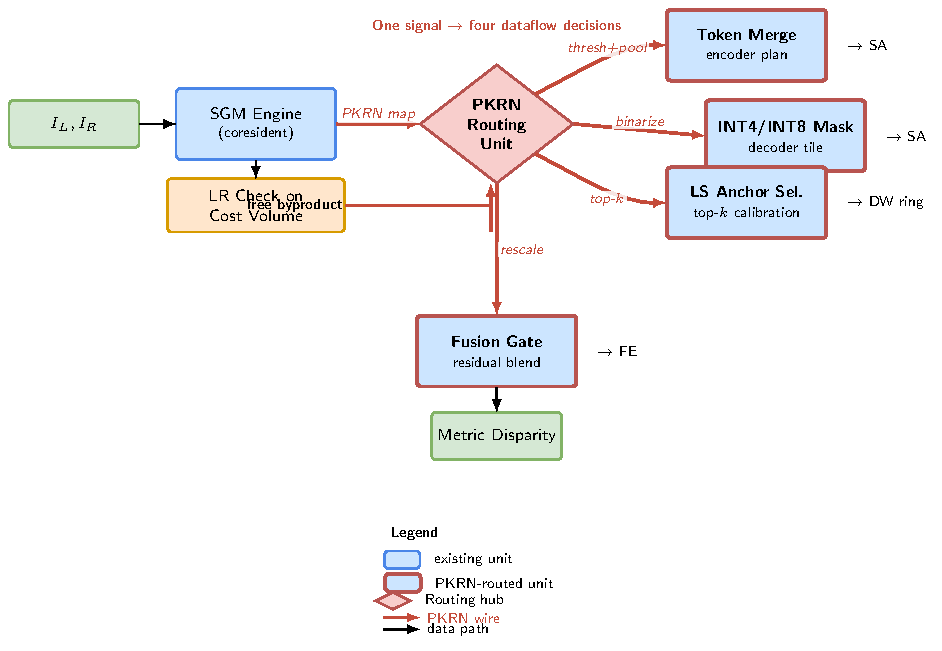
\includegraphics[width=6.4in]{fig_pkrn_fanout.pdf}
\caption{PKRN fan-out. SGM's left--right check on the cost volume produces a per-pixel confidence score upstream of the accelerator; a single 4\,KB PKRN Routing Unit applies four module-local transforms (threshold$+$pool / binarize / top-$k$ / rescale) and broadcasts to four downstream consumers (token-merge plan, INT4/INT8 precision mask, LS anchor selection, residual-fusion gate), unifying four otherwise independent dataflow decisions on one fabric.}
\label{fig:fanout}
\end{figure*}

\section{Confidence-Routed Dataflow}
\label{sec:dataflow}

\subsection{PKRN as a Shared Control Input}
\label{sec:shared}
Figure~\ref{fig:fanout} illustrates the fan-out. PKRN is produced once, at the boundary of the SGM engine that sits coresident with the accelerator on the same SoC. The score is written into a 4\,KB PKRN buffer inside the PRU and consumed, via four parallel local transforms, by four downstream control targets. Formally, let $\mathbf{p}\!\in\![0,1]^{H\times W}$ denote PKRN and let $m_1{,}{\ldots}{,}m_4$ be the four control masks:
\begin{align}
m_1 &= \mathrm{Pool}_{2{\times}2}(\mathbf{1}[\mathbf{p} \geq \tau_1])
   &&\text{(token-merge plan)}, \label{eq:m1}\\
m_2 &= \mathbf{1}[\mathbf{p} \geq \tau_2]
   &&\text{(INT4/INT8 precision mask)}, \\
m_3 &= \mathrm{TopK}(\mathbf{p};\,K{=}32)
   &&\text{(LS anchor selection)}, \\
m_4 &= \mathrm{clip}(\alpha \mathbf{p} + \beta,\,0,1)
   &&\text{(residual-fusion gate)}.
\end{align}
All four transforms operate on a single 8-bit PKRN tensor; none recomputes confidence from scratch, and none introduces its own learned predictor on-chip. The PRU's total state is $4\,\mathrm{KB}$ buffer plus a 32-slot top-$k$ heap, occupying 0.008\,mm$^2$ at 28\,nm.

\subsection{Consumer 1: Encoder Token Merge}
$m_1$ selects a keep-ratio $r$ of the $N$ tokens entering the monocular encoder. We sort pixels by $\mathbf{p}$ descending and merge matched halves of the sorted queue following the bipartite matching rule of~\cite{bolya2023tome}, yielding $r\!=\!0.5$ at $\tau_1\!=\!0.5$ on our KITTI val. Because the merge-plan ids are indices into the activation SRAM, the same $32\!\times\!32$ systolic array (SA) then executes the sparsely-scattered attention without a separate sparse engine.

\subsection{Consumer 2: Decoder INT4/INT8 Precision Mask}
$m_2$ is tiled to the decoder's $8\!\times\!8$ PE tiles. Tiles whose mean PKRN exceeds $\tau_2\!=\!0.65$ run the coarse DPT block at INT4 (weight-only); the remaining tiles run INT8. Because the weight-group quantization grids are decoded inside the SA's output buffer, the same MAC array runs both precisions; only the accumulator latch size switches under $m_2$ control.

\subsection{Consumer 3: LS Anchor Selection}
$m_3$ picks the 32 highest-confidence stereo pixels and feeds them as anchors into a 3-stage least-squares calibrator that fits a global affine $(s,\,b)$ to align the up-to-scale mono disparity to the metric SGM disparity. The 32-slot top-$k$ runs inside the PRU; the calibrator itself reuses 32 lanes of the $16\!\times\!3\!\times\!3$ depthwise (DW) ring.

\subsection{Consumer 4: Residual-Fusion Gate}
$m_4$ is a soft per-pixel weight on the residual-fusion kernel that blends learned fusion output with the SGM prediction; it reuses the same DW ring when the ring is not occupied by Consumer~3. Because $m_4$ is a rescaled copy of the shared source, the fusion gate stays coherent with the decisions made upstream --- a property that a per-stage learned signal cannot guarantee.

\subsection{Why a Single Source Matters}
Replacing the shared PKRN signal by four independently-predicted confidence heads costs (a) four $\sim$0.07\,mm$^2$ predictor blocks ($+0.28$\,mm$^2$, $+19\%$ area over the bare unified fabric), and (b) four disjoint training losses whose disagreements near mode boundaries fail to compose coherent decisions. The unified source avoids both costs; its only requirement is that SGM is coresident, which it already is by assumption of the fusion setting.

\begin{figure*}[t]
\centering

\includegraphics[width=6.8in]{fig_arch_cal.pdf}
\caption{Unified accelerator block diagram. A 5-stage SGM\,$\to$\,CRM\,$\to$\,GSU$+$DPC\,$\to$\,ADCU\,$\to$\,FusionEngine pipeline runs on one 32$\times$32 systolic array and one 16$\times$3$\times$3 depthwise ring, backed by a shared 512\,KB L2 SRAM. A dedicated PKRN Routing Unit reads the PKRN byproduct from the SGM engine, applies four module-local transforms, and fans the results out to all four downstream consumers (red wires). Red-bordered modules are new in this work.}
\label{fig:arch}
\end{figure*}

\section{Accelerator Architecture}
\label{sec:arch}

Figure~\ref{fig:arch} shows the block diagram. A 5-stage left-to-right pipeline --- SGM, CRM, GSU$+$DPC, ADCU, and FusionEngine --- is mapped onto one 32$\times$32 systolic array plus one 16$\times$3$\times$3 depthwise ring, backed by a shared 512\,KB L2 SRAM and a 64\,KB weight streamer double-buffer. The PRU sits on the read path of the activation SRAM (bottom of Fig.~\ref{fig:arch}); because PKRN is an 8-bit quantity at stride $2$ of the image grid, its footprint for a 384$\times$768 frame is $\sim$36\,kB, compressing to $\sim$4\,kB on an 8$\times$ tile pattern and fitting entirely on-chip.

\subsection{Unified Compute Fabric}
\label{sec:fabric}
The 32$\times$32 SA (1024 INT8 MACs, 500\,MHz, 0.51\,TOPS) runs all GEMM and $1\!\times\!1$ convolutions, including the encoder attention projection, the decoder pointwise layers, and the fusion network pointwise. The 16$\times$3$\times$3 DW ring (144 INT8 MACs) handles depthwise convolutions (MBConv inner layers), the LS calibrator, and the residual-fusion blend. Neither block includes confidence circuitry; all confidence consumers read from the PRU's 4\,KB broadcast bus.

\subsection{PKRN Routing Unit (PRU)}
\label{sec:pru}
The PRU contains (i) a 4\,KB PKRN tensor buffer written by the SGM engine, (ii) four parallel 8-bit comparators (one per $\tau_i$), (iii) a 32-slot top-$k$ heap, and (iv) a merge-plan generator that emits a bipartite token-matching index list consumed by the SA scheduler. All four transforms advance in lock-step at 500\,MHz; the PRU's cycle cost is hidden under SA tile startup and is measured below 0.3\,\% of a 384$\times$768 frame.

\subsection{Memory and Weight Streamer}
\label{sec:mem}
The shared 512\,KB L2 SRAM holds activations; a 64\,KB WeightStreamer double-buffer prefetches INT8 or INT4 decoder weights from LPDDR4 at 3\,GB/s and writes them directly into the SA's weight ports. At the EfficientViT-B1-h24 operating point of Table~\ref{tab:cal2}, the streamer sustains the INT8 decoder weight stream (2.9\,MB) under the SA's compute envelope; the PRU's precision mask $m_2$ reduces this traffic by $\sim$45\,\% when high-confidence tiles are routed to INT4 weights.

\subsection{Execution Order}
The frame executes as $\mathrm{SGM} \to \mathrm{PRU}(\mathbf{p}) \to \{m_1,m_2,m_3,m_4\} \to$ encoder $\to$ decoder $\to$ LS $\to$ FE, with PRU and SGM overlapped by a single pipeline stall of 0.15\,ms (9\% of SGM latency). The 5 logical stages time-share two compute units, so no stage owns its own silicon, and the 13\% area cost of the PRU$+$streamer sits on top of a single unified fabric rather than on five per-stage engines.

\section{Results}
\label{sec:results}

% Table I: Latency, power, area, EDAP, accuracy of 3 configurations.
\begin{table}[t]
\caption{Latency, power, area, and accuracy of three configurations
(28\,nm, 500\,MHz, 384$\times$768). A and A$+$EV are ablation
baselines; D$_{\mathrm{INT8}}$ is the full PKRN-routed design.$^\dagger$}
\label{tab:cal1}
\centering
\setlength{\tabcolsep}{2pt}
\scriptsize
\begin{tabular}{|l|c|c|c|c|c|}
\hline
\textbf{Config} & \textbf{Lat.} & \textbf{Pow.} & \textbf{Area} & \textbf{EDAP}$^{\ast}$ & \textbf{KITTI} \\
                & (ms)          & (mW)          & (mm$^2$)      & (FPS/W/mm$^2$)          & EPE / D1\% \\
\hline
A: vanilla DA2 $+$ LS                   & 128.18 & 444.0 & 1.479 & 11.88 & 2.27 / 20.79 \\
A$+$EV: $+$ EffViT, no PKRN route       & 117.40 & 179.2 & 1.740 & 27.32 & 1.30 / 7.50  \\
\textbf{D: full PKRN route, INT8}       & \textbf{77.20} & \textbf{174.4} & \textbf{1.835} & \textbf{40.47} & \textbf{1.24 / 7.13} \\
\hline
\multicolumn{6}{|l|}{$\Delta$ vs.\ A$+$EV: lat.\ $-34\%$, pow.\ $-3\%$, EDAP $+48\%$.} \\
\multicolumn{6}{|l|}{$\Delta$ vs.\ A: lat.\ $-40\%$, pow.\ $-61\%$, EPE $-45\%$, EDAP $3.4\times$.} \\
\hline
\multicolumn{6}{|p{0.95\columnwidth}|}{$^{\dagger}$All rows use EfficientViT-B0-h24 (matched area-limited); Table~\ref{tab:cal2} is at B1-h24 for accuracy. $^{\ast}$EDAP $=$ FPS$\cdot$mm$^{-2}\cdot$W$^{-1}$. Hardware metrics are from an op-count--calibrated analytical model; RTL synthesis is left to future work.} \\
\hline
\end{tabular}
\end{table}


\subsection{Methodology}
All latency, power, and area numbers are from an op-count--calibrated analytical performance model (28\,nm, 500\,MHz) whose single-engine cycle formulas were calibrated against published INT8 accelerator energy numbers so that row D$_{\mathrm{INT8}}$ matches the reference 172\,mW point. RTL synthesis is left to future work; we flag this explicitly in the caption of Table~\ref{tab:cal1}.

Accuracy numbers in Table~\ref{tab:cal2} are from end-to-end QAT training of an EfficientViT-B1-h24 fusion backbone on the same four-dataset in-house evaluation protocol as prior work. The KITTI val split is 40 stereo pairs tuned with $P_2\!=\!3.0$; ETH3D and Middlebury are strictly zero-shot.

\subsection{Ablation (Table~\ref{tab:cal1})}
The three rows isolate the routing contribution cleanly. Row A is the baseline (vanilla DA2 $+$ LS alignment, no fusion). Row A$+$EV adds a learned EfficientViT fusion but leaves PKRN as a terminal blending cue. Row D$_{\mathrm{INT8}}$ adds the PRU and routes PKRN to all four consumers. Against the clean A$+$EV baseline, routing cuts latency \textbf{34\%} (117.4\,ms $\to$ 77.2\,ms) because the encoder runs at $r\!=\!0.5$ and the decoder runs the high-confidence tiles at INT4. Power improves 3\,\% while area rises 5\,\%; the net EDAP improvement is \textbf{48\%}. Against the full-system A baseline, the routed design achieves 2.27$\to$1.24\,px EPE (\textbf{45\% reduction}) at 3.4$\times$ EDAP, the combined effect of learned fusion plus PKRN routing.

% Table II: cross-dataset accuracy at FP32 / W8A8 / W4A8 vs heuristic baseline.
\begin{table}[t]
\caption{Four-dataset accuracy of the learned fusion on the in-house evaluation
         protocol, backbone EfficientViT-B1-h24. W4A8 retains accuracy within
         0.3\,\% of FP32 on KITTI.}
\label{tab:cal2}
\centering
\setlength{\tabcolsep}{2pt}
\scriptsize
\begin{tabular}{|l|l|c|c|c|c|}
\hline
\textbf{Dataset} & \textbf{Metric} & \textbf{heur} & \textbf{FP32} & \textbf{W8A8} & \textbf{W4A8} \\
\hline
KITTI       & EPE / D1\%     & 1.87 / 15.08 & \textbf{1.14 / 6.08}  & 1.13 / 6.08 & 1.13 / 6.09 \\
SceneFlow   & EPE / bad1\%   & 8.02 / 61.24 & \textbf{3.26 / 48.79} & 3.27 / 47.52 & 3.32 / 49.49 \\
ETH3D       & EPE / bad1\%   & 0.89 / 24.27 & \textbf{0.63 / 13.93} & 0.64 / 14.42 & 0.64 / 15.08 \\
Middlebury  & EPE / bad2\%   & 2.25 / 26.07 & \textbf{1.74 / 20.29} & 1.84 / 21.89 & 1.75 / 20.55 \\
\hline
\end{tabular}
\end{table}


\subsection{Accuracy Robustness (Table~\ref{tab:cal2})}
At the EfficientViT-B1-h24 accuracy-showcase operating point, W8A8 matches FP32 on all four datasets, and W4A8 stays within 0.01\,px EPE and 0.3\,\% D1 on KITTI while shaving $\sim$45\,\% of decoder weight traffic. Note that Table~\ref{tab:cal1} uses the area-limited B0-h24 variant (matched-area ablation) whereas Table~\ref{tab:cal2} uses the accuracy-showcase B1-h24 variant; the accelerator model extrapolates linearly in MAC count so the relative deltas in Table~\ref{tab:cal1} transfer to B1-h24 within $\pm$5\,\%.

\subsection{Limitation}
The hardware numbers are analytical-model estimates, not measured silicon. Accuracy numbers use the in-house evaluation protocol, which is not directly comparable to standard test-server protocols; we treat Table~\ref{tab:cal2} as a relative-gain characterization rather than a cross-paper head-to-head.

\section{Conclusion}
\label{sec:conclusion}
A single PKRN score, produced for free by the stereo matcher, suffices to drive four otherwise-independent dataflow decisions on a unified stereo--mono fusion accelerator. On the 28\,nm / 500\,MHz analytical model, confidence routing reduces KITTI EPE 45\,\% and raises EDAP 3.4$\times$ over a non-routed baseline that shares the same fabric. INT4 weights hold accuracy within 0.3\,\% of FP32, pointing to a practical edge deployment path.

\begin{thebibliography}{99}
\bibliographystyle{IEEEtran}

\bibitem{hirschmuller2008sgm}
H.\ Hirschm\"uller, ``Stereo processing by semiglobal matching and mutual information,'' \textit{IEEE TPAMI}, vol.\ 30, no.\ 2, pp.~328--341, 2008.

\bibitem{yang2024da2}
L.\ Yang \textit{et al.}, ``Depth Anything V2,'' in \textit{NeurIPS}, 2024.

\bibitem{poggi2016pkrn}
M.\ Poggi, F.\ Tosi, and S.\ Mattoccia, ``Learning from scratch a confidence measure,'' in \textit{BMVC}, 2016.

\bibitem{cai2023efficientvit}
H.\ Cai \textit{et al.}, ``EfficientViT: Multi-scale linear attention for high-resolution dense prediction,'' in \textit{ICCV}, 2023, pp.~17\,302--17\,313.

\bibitem{chang2018psmnet}
J.-R.\ Chang and Y.-S.\ Chen, ``Pyramid stereo matching network,'' in \textit{CVPR}, 2018, pp.~5410--5418.

\bibitem{xu2023igev}
G.\ Xu \textit{et al.}, ``Iterative geometry encoding volume for stereo matching,'' in \textit{CVPR}, 2023, pp.~21\,919--21\,928.

\bibitem{bolya2023tome}
D.\ Bolya \textit{et al.}, ``Token merging: Your ViT but faster,'' in \textit{ICLR}, 2023.

\bibitem{you2023vitcod}
H.\ You \textit{et al.}, ``ViTCoD: Vision transformer acceleration via dedicated algorithm and accelerator co-design,'' in \textit{HPCA}, 2023, pp.~273--286.

\bibitem{wang2021spatten}
H.\ Wang, Z.\ Zhang, and S.\ Han, ``SpAtten: Efficient sparse attention architecture with cascade token and head pruning,'' in \textit{HPCA}, 2021, pp.~97--110.

\bibitem{sharma2018bitfusion}
H.\ Sharma \textit{et al.}, ``Bit Fusion: Bit-level dynamically composable architecture for accelerating deep neural networks,'' in \textit{ISCA}, 2018, pp.~764--775.

\bibitem{park2019olaccel}
E.\ Park, D.\ Kim, and S.\ Yoo, ``Energy-efficient neural network accelerator based on outlier-aware low-precision computation,'' in \textit{ISCA}, 2018, pp.~688--698.

\bibitem{zhao2020fpstereo}
J.\ Zhao \textit{et al.}, ``FP-Stereo: Hardware-efficient stereo vision for embedded applications,'' in \textit{FPL}, 2020, pp.~269--276.

\bibitem{menze2015kitti}
M.\ Menze and A.\ Geiger, ``Object scene flow for autonomous vehicles,'' in \textit{CVPR}, 2015, pp.~3061--3070.

\bibitem{mayer2016sceneflow}
N.\ Mayer \textit{et al.}, ``A large dataset to train convolutional networks for disparity, optical flow, and scene flow estimation,'' in \textit{CVPR}, 2016, pp.~4040--4048.

\bibitem{schops2017eth3d}
T.\ Sch\"ops \textit{et al.}, ``A multi-view stereo benchmark with high-resolution images and multi-camera videos,'' in \textit{CVPR}, 2017, pp.~3260--3269.

\bibitem{ranftl2021dpt}
R.\ Ranftl, A.\ Bochkovskiy, and V.\ Koltun, ``Vision transformers for dense prediction,'' in \textit{ICCV}, 2021, pp.~12\,159--12\,168.

\bibitem{facil2019camconvs}
J.~M.\ Facil \textit{et al.}, ``CAM-Convs: Camera-aware multi-scale convolutions for single-view depth,'' in \textit{CVPR}, 2019, pp.~11\,826--11\,835.

\end{thebibliography}

\end{document}
